
\documentclass[11pt]{article}


\setlength{\oddsidemargin}{0.0in}
\setlength{\evensidemargin}{0.0in}
\setlength{\topmargin}{0.0in}
\setlength{\topskip}{0.5in}
\setlength{\headheight}{0.5in}
\setlength{\headsep}{0in}
\setlength{\textwidth}{6.5in}
\setlength{\textheight}{8.0in}
\setlength{\parindent}{0in}
\setlength{\parskip}{0.1in}

\setcounter{secnumdepth}{4}
\setcounter{tocdepth}{4}

% \usepackage{times}
\usepackage{fancyvrb}
\usepackage{relsize}
\usepackage{hyperref}
\usepackage{graphicx}
\usepackage{color}
\usepackage{listings}

% theorems, etc.
\usepackage{amsmath}
\newtheorem{theorem}{Theorem}
\newcommand{\BlackBox}{\rule{1.5ex}{1.5ex}}  % end of proof
\newenvironment{proof}{\par\noindent{\bf Proof\ }}{\hfill\BlackBox\\[2mm]}
\newtheorem{lemma}[theorem]{Lemma}
\newtheorem{proposition}[theorem]{Proposition}
\newtheorem{remark}[theorem]{Remark}
\newtheorem{corollary}[theorem]{Corollary}
\newtheorem{definition}[theorem]{Definition}
\newtheorem{conjecture}[theorem]{Conjecture}
\newtheorem{axiom}[theorem]{Axiom}

% for problem sets, each problem automatically numbered
\newcounter{problemnum}
\newcommand{\oneproblem}
   { \stepcounter{problemnum} {\bf \arabic{problemnum}}. } 
\newcommand{\startproblemset}
   { \bigskip {\bf\large Exercises} \setcounter{problemnum}{0} }

\lstset{language=r}
\lstset{
    literate={~} {$\sim$}{1}
}
\lstset{basicstyle=\ttfamily}


 

\begin{document} 

\title{Mixture and Hidden Markov Models: a Unified Introduction}
\author{Norman Matloff \\
   Department of Computer Science \\
   University of California, Davis}

\maketitle

The notion of \textit{mixture distributions} is a classical
probabilistic concept, and arises frequently in applications.  The field
of \textit{Hidden Markov Models} (HMMs) is more ``modern'' on the scale
of the history of probabilistic models; HMMs too have very interesting
applications, such as in bioinformatics and language processing.

As there is a natural connection of mixture models (MMs) to HMMs, we
present both here.  We also present examples of using R packages to
apply these models to data.

We will cover some mathematical detail, but subject to the goal of
keeping things simple.  In the HMM case in particular, derivations
generally involve some famous algorithms that are tedious to follow.
They consist of some clever algebraic manipulations of complex
expressions involving conditional probabilities, which will not be
covered here.

\section{Introduction}

Here we will present two examples, and then give an overview of what MMs
and HMMs do.

\subsection{First Motivating Example:  Network Noise}

Suppose we have a network line that is known to occasionally be
noisy, and that during noisy periods bits will be corrupted in such
a way that the probability of a 0, which is 0.5 in the original
transmitted data, is 0.20 during noisy periods.  Suppose that on average
10\% of the bits arrive during noise periods.

\subsection{Second Motivating Example:  Old Faithful Geyser}

The data here consist of durations of eruptions of the famous
Old Faithful geyser in the US' Yellowstone National Park.  The dataset
here is \textbf{faithful}, a built-in dataset in R.

A histogram, obtained via 

\begin{lstlisting}
> hist(faithful$eruptions)
\end{lstlisting}

and shown in Figure \ref{faithfulhist}, seems to suggest that the
eruption duration distribution is a mixture of two normally distributed random
variables.  This seems even more plausible if we use R's 
\textbf{density()} function, as in Figure \ref{faithfulhistsmooth}.

This has led to many physical theories over the years.  Rather elaborate
physical models have been developed, such as that in O'Hara and Esawi,
Model for the eruption of the Old Faithful geyser, Yellowstone National
Park, \textit{GSA Today}, June 2013.  This paper is full of physical
detail (``... the dynamics of vapor bubble formation (and collapse)
during boiling in the conduit...''), but in simple terms, it posits two
processes, which gave rise to long and short durations before an
eruption, consistent with the bimodal density form suggested by the
above graphs.

\begin{figure}[tb]
\centerline{
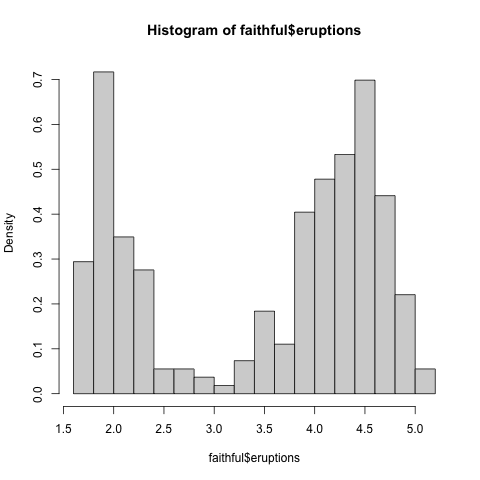
\includegraphics[width=3.0in]{FaithfulDuration.png}
}
\caption{Old Faithful eruption times}
\label{faithfulhist}
\end{figure}

\begin{figure}[tb]
\centerline{
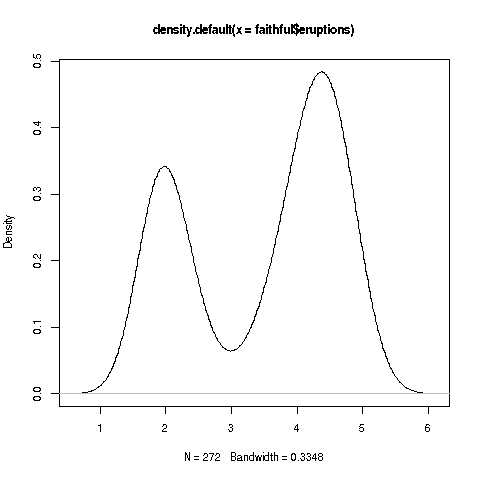
\includegraphics[width=3.0in]{FaithfulDurationSmooth.png}
}
\caption{Old Faithful eruption times, smoothed}
\label{faithfulhistsmooth}
\end{figure}

\subsection{``Hidden'' States}

In the network example, the hidden state is whether we are currently in
a clear period (coded 1) or a noisy period (coded 2).  The observed
state is the actual received bit.

For the purposes of the discussion here, let's take as our geyser model
that of O'Hara \textit{et al} cited above.  Our \textit{hidden}, i.e.\
unknown, state here will be the identity of the currently eruption type,
long (coded 1) or short (coded 2) Our \textit{observed} state is the
duration of the eruption.  Note the overlap: some durations
for type 1 eruptions may actually be shorter than some durations
for eruptions of type 2.

In many applications, a major part of the modeling process is deciding
on the number of states.  In our two models above, it is natural to take
this number to be 2, but generally there is no obvious such number.  In
such cases, we have a classic model-fitting choice, the famous
\textit{Bias-Variance Tradeoff}:  The more hidden states in our model,
the smaller the bias (in the form of inaccuracy of the model itself) but
the larger the variance (sampling error); setting the number of hidden
states at too large a level will result in overfitting.

\subsection{``Time''}

In some applications, time is really time.  If our data is stock price,
say, we have Day 1, Day 2, Day 3 and so on.  In other applications,
``time'' is an index, such at Bit 1, Bit 2, Bit 3 etc.

In the case of MMs, most applications do not have a time component at
all.  Examples will be given, but we first use the geyser example, which does
have a time component, so as to best illustrate the commonality between
MMs and HMMs.

\subsection{Conditional Probabilities of Observed Values}

Let $S_i$ denote the hidden state at time $i$, 
and let $Y_i$ denote the corresponding observed value.  A key ingredient
in the analysis will be expressions of the form

\begin{equation}
P(Y_i = w | S _i = v)
\end{equation}

If $Y$ is continuous rather than discrete, the above expression would be
something like

\begin{equation}
f_{Y|S} (w,v) 
\end{equation}

where $f_{Y|S}$ is the conditional density of $Y$ given $S$.

These conditional distribution quantities are then used to estimate
model parameters, as we will see below.

\subsection{Mixture Models vs.\ HMMs: the 10,000 Foot View}

Both types of models have hidden and observed states.  But HMMs add an
extra aspect:  We model the system as evolving in time, with
probabilities of going from one state to another at each time step.  So
this is a dynamic model, while MMs are usually static. 

In the Old Faithful example, for instance, in an MM we may wish to
estimate the overall proportion of eruptions of type 1, while in an
HMM we may wish to have an estimated probability that the \textit{next}
eruption is of that type.

\section{Mixture Models}

Actually, MMs are typically not presented in the conditional distribution
form we saw above.  Let's see how to reconcile the standard description
with what we saw above.

\subsection{Definition}

Say $Y$ is discrete.  Then

\begin{equation}
P(Y = w) = \sum_{v} P(S = v) ~ P(Y = w | S = v)
\end{equation}

So in terms of cumulative distribution functions (cdfs),

\begin{equation}
F_Y(w) = P(Y \leq w) = 
\sum_{v} P(Y \leq w | S = v) ~ P(S = v) =
\sum_{v} c_v F_{Y|S}(w,v)
\end{equation}

where 

\begin{equation}
c_v = P(S = v)
\end{equation}

and $F_{Y|S}$ is the conditional distribution of $Y$ given $S$.

Speaking just in terms of cdfs, we say that $F_Y$ is a \textit{mixture}
of the cdfs $F_{Y|S}$, which simply means that $F_Y$ is a linear
combination of the $F_{Y|S}$, where the coefficients are nonnegative
numbers whose sum is 1.

Consider random variables $X_1,...,X_k$, with cumulative distribution
functions $F_{X_i}$ (not necessarily independent), and let $c_i, ~
i=1,...,k$ be nonnegative numbers whose sum is 1.  Define the random
variable $M$ to take on the value $X_i$ with probability $c_i$,
$i=1,...,k$.  Then we say that $M$ has a mixture distribution.
With this view, the state is only implicit.

Note that

\begin{equation}
F_{M}(t) = \sum_{i=1}^k c_i F_{X_i}(t)
\end{equation}

Similar relations hold for probability mass functions ($X_i$ discrete)
and density functions ($X_i$ continuous).

In MM analysis, the usual quantities of interest are the 
$F_{X_i}$ and the $c_i$.  In the Old Faithful example, the former 
typically means using the data to somehow estimate the means and
standard deviations of the two normal distributions, and the proportions
of eruptions of the two types.

Probably the most common approach to estimating such quantities is the
\textit{EM algorithm}.  We will present the details in Section
\ref{emalg}, but will make use of it now.

\subsection{The mixtools Package}

This is a large package with many functions for analysis of MMs.  The EM
algorithm is used extensively.  Here we will illustate the function
\textbf{normalmixEM()}, which as the name implies, fits an MM of normal
distributions.  Again, for the sake of simplicity, we will cover only a
few of the many features of this function.

I tried initial guesses of means and standard deviations from the
appearance of the histogram, and used equal weights for my initial
guesses in that aspect:

\begin{lstlisting}
> mixout <- normalmixEM(faithful$eruptions,lambda=0.5,mu=c(55,80),sigma=10,k=2)
number of iterations= 9 
> str(mixout)
List of 9
 $ x         : num [1:272] 79 54 74 62 85 55 88 85 51 85 ...
 $ lambda    : num [1:2] 0.361 0.639
 $ mu        : num [1:2] 54.6 80.1
 $ sigma     : num [1:2] 5.87 5.87
 $ loglik    : num -1034
 $ posterior : num [1:272, 1:2] 1.02e-04 1.00 4.12e-03 9.67e-01 1.21e-06
...
  ..- attr(*, "dimnames")=List of 2
  .. ..$ : NULL
  .. ..$ : chr [1:2] "comp.1" "comp.2"
 $ all.loglik: num [1:10] -1085 -1051 -1037 -1034 -1034 ...
 $ restarts  : num 0
 $ ft        : chr "normalmixEM"
 - attr(*, "class")= chr "mixEM"
\end{lstlisting}

So, the estimate from EM is that about 36\% of the eruptions are of Type
1, etc.  Interesting, when I tried it without my own initial guesses,

\begin{lstlisting}
mixout <- normalmixEM(faithful$eruptions,k=2)
\end{lstlisting}

the results were the same, so it seems to be a fairly stable model here.

By the way, since we are working with a hidden variable M here---in
fact, we are merely postulating that it exists---how do we check this
assumption?  We'll return to this general idea of model fitting in
Chapter \ref{chap:mod}.

\subsection{Mean and Variance of Random Variables Having Mixture
Distributions}
\label{mixmeanvar}

Think of the random variables M and Y in the discussion following
(\ref{continmix}).  Then EY is easy to find using the Law of Total
Expectation:

\begin{equation}
\label{mixmean}
EY = E[E(Y | M)]
\end{equation}

Of course, evaluating this would require being able to compute E(Y $|$
M), which is easy in some cases, not so easy in others.

Also, using the Law of Total Variance, we have that

\begin{equation}
\label{mixvar}
Var(Y) = E[Var(Y|M)] + Var[E(Y|M)]
\end{equation}

\section{Hidden Markov Models}

\section{More on Mixtures};

\subsection{The EM Algorithm}
\label{emalg}

Now returning to our main topic of mixture models, let's discuss a very
common tool for fitting such models.

Consider again the example in Section \ref{oldtrick}.  Now suppose p, q
and r are all unknown, and we wish to estimate them from data. Say we
will perform the above experiment 50 times, resulting in our data
$N_1,...,N_{50}$ We will estimate p, q and r by applying some method,
say the Method of Moments, Maximum Likelihood or some ad hoc method of
our own, to our data. Each $N_i$ has the distribution seen in $p_N$
above. This is a parametric family, with 3 parameters. (If, say, r is
known, we only have a two-parameter family, and things are easier.)

So, how can we estimate those three parameters?  In Chapter
\ref{chap:est}, we found some general methods for parameter estimation.
Let's look at one of them, Maximum Likelihood Estimators (MLEs).

In (\ref{mixbinom}), the MLE vector 
$(\widehat{p},
  \widehat{q},
  \widehat{r})'$
would be found by maximizing

\begin{equation}
\Pi_{i=1}^n
\left [ r \binom{10}{N_i} p^{N_i} (1-p)^{10-N_i} +
(1-r) \binom{10}{N_i} q^{N_i} (1-q)^{10-N_i}
\right ]
\end{equation}

After taking derivatives, etc., one would end up with a messy, nonlinear
set of equations to solve.  One could try {\bf mle()}, but there is a
better way to get the MLE: the Expection/Maximization (EM) algorithm.
The derivation and ultimate formulas can get quite complex.
Fortunately, R libraries exist, such as {\bf mixtools}, so you can avoid
knowing all the details, as long as you understand the basic notion of a
mixture model.  

In something like (\ref{hsum}), for instance, one would make initial
guesses for the $p_M(i)$ and then estimate the parameters of the $g_i$.
In the next step, we'd do the opposite---take our current guesses for
the latter parameters as known, and estimate the $p_M(i)$.  Keep going
until convergence.

To make things concrete, recall the trick coin example Section
\ref{oldtrick}.  But change it a little, so that the probabilities of
heads for the two coins are unknown; call them $p_0$ (heads-light coin)
and $p_1$ (heads-heavy coin).  And also suppose that the two coins are
not equally likely to be chosen, so that $p_M()$ is not known; denote
P(M = 1) by q.

Suppose we have sample data, consisting of doing this experiment
multiple times, say by reaching into the box n times and then doing m
flips each time.  We then wish to estimate 3 quantities---q and the two
$p_i$---using our sample data.  

We do so using the following iterative process.  (The account here is
not exactly EM, but captures the spirit of it.) We set up initial
guesses, and iterate until convergence:

\begin{itemize}

\item {\bf E step:} Update guess for q (complicated Bayes Rule equations).

\item {\bf M step:} Using the new guess for q, update the gueses for the
two $p_i$.

\end{itemize}

The details are beyond the scope of this book.\footnote{``M'' in the M
step refers to the Maximum Likelihood method, a special case of the
material in Section \ref{mle}.}

\subsection{Example:  Two Kinds of Batteries}

Say a factory produces two kinds of batteries.  One kind has lifetime
that is exponentially distributed with mean 200 and the other's
distribution is exponential with mean 500.  Suppose 60\% of the
factory's production is of the former type, with 40\% being of the
latter type.  Let's find the mean and variance of the lifetime Y of a
randomly chosen battery.

Note that the distribution of Y is a mixture, in the sense of Section
\ref{genmix}, in particular (\ref{continmix}).  Y here is a continuous
random variable, referred to in that section as the ``continuous
outcome'' case.   In the notation there, let M be the battery type, with
M being 0 or 1, for the 200-hour and 500-hour batteries, respectively.
The conditional density of Y given M = 0 is exponential with mean 200,
while given M = 1 it is exponential with mean 500.  The unconditional
density of Y is the mixture of these two exponential densities, as 
(\ref{continmix}).

We want to find the \underline{un}conditional mean and variance of Y.

Then

\begin{equation}
\label{batt1}
E(Y|M)=\left\{ \begin{array}{rl}
200, & w.p. ~ 0.60 \\
500, & w.p. ~ 0.40
\end{array}\right. 
\end{equation}

and 

\begin{equation}
\label{batt2}
Var(Y|M)=\left\{ \begin{array}{rl}
200^2, & w.p. ~ 0.60 \\
500^2, & w.p. ~ 0.40
\end{array}\right. 
\end{equation}

(recalling that in the exponential family, variance is the square of the
mean).

We can now use the formulas in Section \ref{mixmeanvar}.  Let $Q_1 =
E(Y|M)$  and $Q_2 = Var(Y|M)$.  Then

\begin{equation}
EY = EQ_1 = 0.60 \times 200 + 0.40 \times 500
\end{equation}

and 

\begin{eqnarray}
Var(Y) &=& E(Q_2) + Var(Q_1) \\
&=& (0.60 \times 200^2 + 0.40 \times 500^2) + Var(Q_1) \\
&=& (0.60 \times 200^2 + 0.40 \times 500^2) + E(Q_1^2) - (EQ_1)^2 \\
&=& (0.60 \times 200^2 + 0.40 \times 500^2) + (0.60 \times 200^2 + 0.40
\times 500^2)  \\
& & - (0.60 \times 200 + 0.40 \times 500)^2 \\
\end{eqnarray}

\subsection{Example:  Overdispersion Models}

A common model used in practice is that of {\bf overdispersion}, in
connection with Poisson models.  

Recall the following about the Poisson distribution family:

\begin{itemize}

\item [(a)] This family is often used to model counts.

\item [(b)] For any Poisson distribution, the variance equals the mean.

\end{itemize}

In some cases in which we are modeling count data, condition (b) is too
constraining.  We want a ``Poisson-ish''
distribution in which the variance is greater
than the mean, called {\bf overdispersion}.  

One may then try to fit a mixture of several Poisson distributions,
instead of a single one.  This does induce overdispersion, as we will
now see.  

Suppose M can equal 1,2,...,k, with probabilities $p_1,...,p_k$ that sum
to 1.  Say the distribution of Y given M = i is Poisson with parameter
$\lambda_i$.  Then Y has a mixture distribution.  Our goal here will be
to show that Y is overdispersed, i.e. has a large variance than mean.

By the Law of Total Expectation,

\begin{eqnarray}
\label{meanlamb}
EY &=& E[E(Y|M)] \\ 
&=& E(\lambda_M) \label{elambm} \\
&=& \sum_{i=1}^k p_i \lambda_i
\end{eqnarray}

Note that in the above, the expression $\lambda_M$ is a random variable,
since its subscript M is random.  Indeed, it is a function of M, so
Equation (\ref{egofx}) then applies, yielding the final equation.  The
random variable $\lambda_M$ takes on the values $\lambda_1,...,\lambda_k$
with probabilities $p_1,...,p_k$, hence that final sum.

The corresponding formula for variance, (\ref{bis}), can be used to
derive Var(Y).

\begin{eqnarray}
Var(Y) &=& E[Var(Y|M)] + Var[E(Y|M)] \\ 
&=& E(\lambda_M) + Var(\lambda_M) \label{thislast} \\
&=& EY + Var(\lambda_M) \label{thislast} \\
\end{eqnarray}

Did you notice that this last equation achieves our goal of showing
overdispersed?  Since

\begin{equation}
Var(\lambda_M) > 0
\end{equation}

we have that

\begin{equation}
Var(Y) > E(\lambda_M) = EY
\end{equation}

by (\ref{elambm}).

But let's see just how much greater the variance is than the mean.  The
second term in (\ref{thislast}) is evaluated the same way as in
(\ref{elambm}):  This is the variance of a random variable that takes on
the values $\lambda_1,...,\lambda_k$ with probabilities $p_1,...,p_k$,
which is

\begin{equation}
\sum_{i=1}^k p_i (\lambda_i - \overline{\lambda})^2
\end{equation}

where 

\begin{equation}
\overline{\lambda} =  E\lambda_M = \sum_{i=1}^k p_i \lambda_i
\end{equation}

Thus

\begin{equation}
EY = \overline{\lambda}
\end{equation}

and

\begin{equation}
Var(Y) = \overline{\lambda} + 
\sum_{i=1}^k p_i (\lambda_i - \overline{\lambda})^2
\end{equation}

So, as long as the $\lambda_i$ are not equal, we have

\begin{equation}
Var(Y) > EY
\end{equation}

in this Poisson mixture model, in contrast to the single-Poisson case
in which Var(Y) = EY.  You can now see why the Poisson mixture model is
called an overdispersion model.

So, if one has count data in which the variance is greater than the
mean, one might try using this model.

In mixing the Poissons, there is no need to restrict to discrete M.  In
fact, it is not hard to derive the fact that if X has a gamma
distribution with parameters r and p/(1-p) for some $0 < p < 1$, and Y
given X has a Poisson distribution with mean X, then the resulting Y
neatly turns out to have a negative binomial distribution.

% Again, there may be a computability issue.  But see the examples below.

% \section{Example:  Cluster Analysis}
% 
% We will in Section \ref{mixclust} see that the notion of mixtures can
% also be applied to clustering.
% 
% \section{Markov Chain with Random $X_0$}
% 
% LOSE MARKOV PROPERTY
% 
% \section{Bayes Models, Including Empiricial Bayes}
% 
% JUST REFER TO THE BAYES SECTION, BUT NOTE IN THE LATTER THAT IT IS A
% MIXTURE

% \section{De Finetti's Theorem}
% 
% Consider again the trick coin example, Section \ref{oldtrick}.  As we
% have discussed, the tosses $B_i$ are not independent.  However, they are
% {\bf exchangeable}:
% 
% \begin{equation}
% P(B_
% \end{equation}


\end{document}

> x <- geyserSim(100000,0.9,0.3)
> z <- hmmr::hmm(x,2)
> summary(z)
Initial state probabilities model
pr1 pr2
  1   0

Transition matrix
        toS1  toS2
fromS1 0.681 0.319
fromS2 0.891 0.109

Response parameters
Resp 1 : gaussian
    Re1.(Intercept) Re1.sd
St1          -0.016  0.991
St2           1.959  1.018

geyserSim <- function(nTimePers,AtoB,BtoA)
{
   x <- vector(length=nTimePers)
   state <- 'A'
   for (i in 1:nTimePers) {  # could use rgeom() and while{} instead
      # check for state change
      if (state == 'A') {
         if (runif(1) < AtoB)  # now bad network
            state <- 'B'
      } else {  # state == 'B'
         if (runif(1) < BtoA)  # now bad network
            state <- 'A'
      }
      if (state == 'B') x[i] <- rnorm(1)
      else x[i] <- rnorm(1) + 2
   }
   x
}

netSim <- function(nBits,goodToBadProb,badToGoodProb,badProb0) 
{
   trueBits <- sample(0:1,nBits,replace=TRUE)
   rcvdBits <- trueBits  
   state <- 'good'
   for (i in 1:nBits) {  # could use rgeom() and while{} instead
      # check for state change 
      if (state == 'good') {
         if (runif(1) < goodToBadProb)  # now bad network
            state <- 'bad'
      } else {  # state == 'bad'
         if (runif(1) < badToGoodProb)  # now bad network
            state <- 'good'
      }
      if (state == 'bad' && runif(1) < badProb0)
         rcvdBits[i] <- 0
   }
   cbind(trueBits,rcvdBits)
}



